
\begin{figure*}[t]
\centering
\begin{subfigure}{0.19\textwidth}
\includegraphics[width=\textwidth]{images/gtannotations/pixmmvp/17.jpg}
\captionsetup{labelformat=empty}
\caption{\tiny{the front of the school bus}}
\end{subfigure}%
\begin{subfigure}{0.19\textwidth}
\includegraphics[width=\textwidth]{images/gtannotations/pixmmvp/19.jpg}
\captionsetup{labelformat=empty}
\caption{\tiny{the dorsal fin of the animal}}
\end{subfigure}%
\begin{subfigure}{0.19\textwidth}
\includegraphics[width=\textwidth]{images/gtannotations/pixmmvp/30.jpg}
\captionsetup{labelformat=empty}
\caption{\tiny{the window on the school bus}}
\end{subfigure}%
\begin{subfigure}{0.19\textwidth}
\includegraphics[width=\textwidth]{images/gtannotations/pixmmvp/41.jpg}
\captionsetup{labelformat=empty}
\caption{\tiny{the spider's legs}}
\end{subfigure}%
\begin{subfigure}{0.19\textwidth}
\includegraphics[width=\textwidth]{images/gtannotations/pixmmvp/48.jpg}
\captionsetup{labelformat=empty}
\caption{\tiny{the spots on the animal}}
\end{subfigure}

\begin{subfigure}{0.19\textwidth}
\includegraphics[width=\textwidth]{images/gtannotations/pixcvbench/000000009400.jpg}
\captionsetup{labelformat=empty}
\caption{\tiny{mouse, keyboard (annotated ... red box)}}
\end{subfigure}\hspace{1em}%
\begin{subfigure}{0.19\textwidth}
\includegraphics[width=\textwidth]{images/gtannotations/pixcvbench/000000007574.jpg}
\captionsetup{labelformat=empty}
\caption{\tiny{bottle}}
\end{subfigure}\hspace{1em}%
\begin{subfigure}{0.2255\textwidth}
\includegraphics[width=\textwidth]{images/gtannotations/pixcvbench/000000014439.jpg}
\captionsetup{labelformat=empty}
\caption{\tiny{chair (annotated by the red box), kite}}
\end{subfigure}\hspace{1em}%
\begin{subfigure}{0.21\textwidth}
\includegraphics[width=\textwidth]{images/gtannotations/pixcvbench/ADE_val_00001312.jpg}
\captionsetup{labelformat=empty}
\caption{\tiny{glass, drinking glass}}
\end{subfigure}
\caption{Examples of ground-truth annotations for referring expressions in the respective object of interest in the question and their segmentation masks. First row: PixMMVP examples, Second row: PixCV-Bench examples. Ground-truth highlighted in green.}
\label{fig:gt}
\end{figure*}

\section{Additional implementation details}
\label{app:impdetails}
In this section, we cover additional details about our proposed datasets and the implementation of the evaluation setup and baselines. We also refer to the output from the questions of the three probing techniques in the supplementary material for all the studied models. 

\textbf{Datasets.} Our proposed datasets, PixMMVP and PixCV-Bench, are composed of ground-truth referring expressions describing the object of interest in the respective question and its segmentation mask. We show in Fig.~\ref{fig:gt} examples of these ground-truth annotations for both datasets. It shows the challenging scenarios in pixel-level visual grounding which is strongly tied to the visual question answering task, since an integral part of answering these questions requires the grounding of the object/s of interest.

\textbf{Models.} We also detail the model checkpoints we use for the four pixel-level MLLMs and their variants, retrieved from HuggingFace~\cite{wolf2019huggingface} in Table~\ref{tab:checkpoints}. These also include the model checkpoints used for the base MLLMs that were not trained with pixel-level visual grounding. It is worth noting, that for GLAMM we use two variants (FullScope and RegCap) since their base model (i.e., FullScope) has low performance in the visual question answering task. As such we use the other variant for GLAMM that was fine-tuned for region-level captioning using RefCOCOg dataset. Furthermore, we provide details on the \textit{oracle} selection mechanism, we discard the cases where the ground-truth segmentation is all background in the when analysis, since there is no ground-truth grounding to evaluate against. These occur in few cases in PixMMVP.

Additionally, we provide details on the SAM model that is used in the three baselines and upper bounds in our benchmarks, where we use the ViT-H variant. Finally, we provide an illustrative example of our automatic selection mechanism with the corresponding predictions on PixMMVP using Llava 1.5 (7B) in Fig.~\ref{fig:auto}. Our automatic selection goes through an iterative process of prompting the selected MLLM, in our case GPT-4o, with groups of images highlighting the predicted segmentation to select the best within each group. In the final stage the best images are used to prompt the MLLM to select the final selected mask that best describes the object of interest.

\begin{table}[t]
\resizebox{0.47\textwidth}{!}{
\begin{tabular}{l|l}
\hline
 \textbf{Model Name} & \textbf{Model Checkpoint}\\ \hline
 LISA &  xinlai/LISA-7B-v1-explanatory \\
 GLAMM & MBZUAI/GLaMM-FullScope \\
 GLAMM-RegCap & MBZUAI/GLaMM-RegCap-RefCOCOg\\
 Llava-G & Haozhangcx/llava\_grounding\_gd\_vp \\
 Llava 1.5 (7B) & liuhaotian/llava-v1.5-7b \\
 Llava 1.5 (13B) & liuhaotian/llava-v1.5-13b \\
 Cambrian-1 (8B) & nyu-visionx/cambrian-8b \\ \hline
\end{tabular}}
\caption{Hugging Face model checkpoints used in our benchmarks.}
\label{tab:checkpoints}
\end{table}

\textbf{Evaluation.} We also provide the details on computing the visual question answering accuracy using GPT-4o in the first protocol~\cite{tong2024eyes}. We use the following prompt: \textit{``Given the following question $<$QUESTION$>$, the correct answer is $<$ANSWER$>$. Does the following answer correctly answers the question, answer: $<$RESPONSE$>$? Respond with a Yes/No''}.

\section{Additional qualitative analysis}
\label{app:qual}
In this section, we provide a qualitative ablation of our baselines and a visualization of the attention maps that can show how vanilla MLLMs are reasoning on the question they are answering. Additionally, we provide qualitative examples showing when grounding emerges in these vanilla MLLMs. Finally, we provide more examples on PixMMVP and PixCV-Bench benchmarks.

\begin{figure*}[t]
\centering
\includegraphics[width=\textwidth]{images/auto.drawio-2.pdf}
\caption{The automatic selection baseline, PixFoundation, which uses a simple mechanism of highlighting the predicted masks in red then prompting a multi-modal large language model to select the right mask from the group of highlighted images, followed by the final mask selection.}
\label{fig:auto}
\end{figure*}

\subsection{Baselines ablation}
We show the qualitative ablation among the two baselines and upper bound using the best base MLLM Cambrian-1 (8B) in Fig.~\ref{fig:appablation} on PixMMVP. The three  confirm that there is grounding emerging in MLLMs that were not trained with pixel-level grounding supervision. Nonetheless, it shows that identifying when that grounding emerges is equally important in retrieving the best segmentation of the referring expression. The first baseline, attend and segment, assumes the alignment between the attention map that can be mined for the segmentation mask and the noun phrase that has the highest correspondence to the ground-truth category or noun phrase. Our findings quantitatively and qualitatively show otherwise, where grounding can emerge in different output tokens. It also shows the \textit{oracle} upper bound for mask selection, PixFoundation$\dagger$, exhibiting better segmentation than the attend and segment, confirming on the aforementioned finding. Additionally, it shows that our simple automatic mechanism, PixFoundation, surpasses the attend and segment as well on PixMMVP.

\begin{figure}[t]
\centering
Attend and Segment~\cite{cao2024emerging} (Cambrian-1 (8B))

\begin{subfigure}{0.12\textwidth}
\includegraphics[width=\textwidth]{images/qualfig2/cambrian_spacy/9.jpg}
\end{subfigure}%
\begin{subfigure}{0.12\textwidth}
\includegraphics[width=\textwidth]{images/qualfig2/cambrian_spacy/10.jpg}
\end{subfigure}%
\begin{subfigure}{0.12\textwidth}
\includegraphics[width=\textwidth]{images/qualfig2/cambrian_spacy/89.jpg}
\end{subfigure}%
\begin{subfigure}{0.12\textwidth}
\includegraphics[width=\textwidth]{images/qualfig2/cambrian_spacy/280.jpg}
\end{subfigure} 

PixFoundation (Cambrian-1 (8B))

\begin{subfigure}{0.12\textwidth}
\includegraphics[width=\textwidth]{images/qualfig2/cambrian_auto/9.jpg}
\end{subfigure}%
\begin{subfigure}{0.12\textwidth}
\includegraphics[width=\textwidth]{images/qualfig2/cambrian_auto/10.jpg}
\end{subfigure}%
\begin{subfigure}{0.12\textwidth}
\includegraphics[width=\textwidth]{images/qualfig2/cambrian_auto/89.jpg}
\end{subfigure}%
\begin{subfigure}{0.12\textwidth}
\includegraphics[width=\textwidth]{images/qualfig2/cambrian_auto/280.jpg}
\end{subfigure}

PixFoundation$\dagger$ (Cambrian-1 (8B))

\begin{subfigure}{0.12\textwidth}
\includegraphics[width=\textwidth]{images/qualfig2/cambrian_oracle/9.jpg}
\caption{}
\end{subfigure}%
\begin{subfigure}{0.12\textwidth}
\includegraphics[width=\textwidth]{images/qualfig2/cambrian_oracle/10.jpg}
\caption{}
\end{subfigure}%
\begin{subfigure}{0.12\textwidth}
\includegraphics[width=\textwidth]{images/qualfig2/cambrian_oracle/89.jpg}
\caption{}
\end{subfigure}%
\begin{subfigure}{0.12\textwidth}
\includegraphics[width=\textwidth]{images/qualfig2/cambrian_oracle/280.jpg}
\caption{}
\end{subfigure}

\caption{Baselines and upper bound ablation using the base MLLM, Cambrian-1 (8B), ablating the different schemes for mask selection. We use the second probing to prompt the MLLM to identify the referred expression. The referring expressions for these examples are as follows: (a) the key ``z'', (b) the key ``z'', (c) people, (d) the elderly person. Predictions are highlighted in red.} 
\label{fig:appablation}
\end{figure}

\begin{figure}[t]
\centering

\begin{subfigure}{0.16\textwidth}
\stackunder[5pt]{\includegraphics[width=\textwidth]{images/appqualattmaps/292_015_att.jpg}}{the yellow skin}
\end{subfigure}%
\begin{subfigure}{0.16\textwidth}
\stackunder[5pt]{\includegraphics[width=\textwidth]{images/appqualattmaps/292_016_att.jpg}}{blue overalls}
\end{subfigure}%
\begin{subfigure}{0.16\textwidth}
\stackunder[5pt]{\includegraphics[width=\textwidth]{images/appqualattmaps/292_017_att.jpg}}{goggles}
\end{subfigure}

\begin{subfigure}{0.16\textwidth}
\stackunder[5pt]{\includegraphics[width=\textwidth]{images/appqualattmaps/107_008_att.jpg}}{six legs}
\end{subfigure}%
\begin{subfigure}{0.16\textwidth}
\stackunder[5pt]{\includegraphics[width=\textwidth]{images/appqualattmaps/107_010_att.jpg}}{the front legs}
\end{subfigure}%
\begin{subfigure}{0.16\textwidth}
\stackunder[5pt]{\includegraphics[width=\textwidth]{images/appqualattmaps/107_012_att.jpg}}{a hairy texture}
\end{subfigure}
\caption{Normalized attention maps visualization showing the noun phrase and its corresponding attention in the output text for two PixMMVP examples using Cambrian-1 (8B) base MLLM. While the attention maps can not be directly used as segmentation, yet it provides initial locations for the maximally attended pixels corresponding to what the model is looking at. In certain scenarios it exactly aligns with the noun phrase describing it as in the two examples. Yet in certain scenarios as we showed earlier, the grounding of the referred expression in question emerges with other noun phrases describing it.}
\label{fig:attmaps}
\end{figure}

\subsection{Attention maps visualization}
In this section, we visualize the normalized attention maps, $\tilde{A}$, in Fig.~\ref{fig:attmaps}. We show two examples for Cambrian-1 (8B) from PixMMVP using the first probing where we directly prompt the model with question and options. The first row shows outstanding ability to visually ground the different noun phrases from the output text. The full output text of the first row example is: \textit{``The image provided is a cake designed to resemble a minion from the \"Despicable Me\" franchise. It is not a living creature and therefore cannot smile or have a tongue out. The cake is an inanimate object, crafted to mimic the appearance of a minion, which is a fictional character from the animated movie series. The design elements such as the \textbf{yellow skin, blue overalls, and goggles} are characteristic of the minions' appearance in the films.''} The visualization shows how the maximally attended locations for the last three noun phrases correspond to the correct locations in the image.

The second output text corresponding to the example shown is; \textit{``The butterfly's feet, also known as tarsi, are not distinctly visible in this image  due to the angle and the butterfly's wings being open. However, we can infer their presence and approximate location. Monarch butterflies have \textbf{six legs}, with the hind legs being the longest and the \textbf{front legs} being the shortest. The legs are typically slender and have a \textbf{hairy texture}, which aids in gripping onto surfaces. In this image, the legs are likely located at the bottom of the butterfly's  body, just below the abdomen, and are probably in contact with the leaf it is perched on.''} The attention maps highlight what we suspect is a failure where the MLLM mistakes the antenna of the butterfly for front legs. Such hidden failures that do not necessarily affect the correctness of the answer, are still important to study and we believe our tool with the \textit{oracle} upper bound can be used to inspect this further. Finally, we find that these attention maps in both examples are not sufficiently accurate to be used for segmentation directly, yet when paired with a powerful segmentation method like SAM it provides a good segmentation performance.

\subsection{When does grounding emerge?}
We show additional examples on when grounding emerges in multi-modal large language models, specifically in the Llava 1.5 (7B) variant, using the second probing to prompt the model to segment what is in the referring expression. Figures~\ref{fig:when1}, \ref{fig:when2}, \ref{fig:when3} and \ref{fig:when4} show the corresponding predicted masks for the grounding that emerged highlighted in red with the maximum attention point as a black dot. Figure~\ref{fig:when_imgs} in the main text shows the aforementioned four examples with the input prompt, the concept category and the noun phrase corresponding to the best grounding using the \textit{oracle} selection and the full output text. It clearly shows that the correct output token can correspond to location or color but not necessarily the ground-truth referring expression. While some of the noun phrases and their masks from the point prompting of SAM do correspond to what the noun phrase is describing. It is not always the case, example in Fig.~\ref{fig:when2} ``the flame'' was not able to highlight the correct object yet it appeared in the noun phrase corresponding to the location ``the top''. It also shows that the majority of correct grounding occurs near the end of the output text after the model reasoned for an answer to the question.

Additionally, this type of mining for attention maps can show potential mistakes that MLLMs fall into while performing the grounding to reason on what is in the image. An example on that is in Fig.~\ref{fig:when4}, where the model potentially mistakes a crack in the wood for the minute hand. Thus, our PixFoundation$\dagger$ serves as an interesting tool to interpret and understand how MLLMs work and reason to produce the final output with the \textit{oracle} selection as an upper bound. Yet, there is an open question on how to identify the real mistake from the MLLM \textit{vs.} simple misalignment between the noun phrase and the grounding emerging, since grounding could emerge with phrases describing it or parts of it instead of the object's noun phrase itself. We leave this for future work.

\begin{figure}[t]
\centering
the image
\begin{subfigure}{0.16\textwidth}
\includegraphics[width=\textwidth]{images/appqualwhen/1_overlays/1_000_000.jpg}
\end{subfigure}%
\begin{subfigure}{0.16\textwidth}
\includegraphics[width=\textwidth]{images/appqualwhen/1_overlays/1_000_001.jpg}
\end{subfigure}%
\begin{subfigure}{0.16\textwidth}
\includegraphics[width=\textwidth]{images/appqualwhen/1_overlays/1_000_002.jpg}
\end{subfigure}

a butterfly
\begin{subfigure}{0.16\textwidth}
\includegraphics[width=\textwidth]{images/appqualwhen/1_overlays/1_001_000.jpg}
\end{subfigure}%
\begin{subfigure}{0.16\textwidth}
\includegraphics[width=\textwidth]{images/appqualwhen/1_overlays/1_001_001.jpg}
\end{subfigure}%
\begin{subfigure}{0.16\textwidth}
\includegraphics[width=\textwidth]{images/appqualwhen/1_overlays/1_001_002.jpg}
\end{subfigure}

orange wings
\begin{subfigure}{0.16\textwidth}
\includegraphics[width=\textwidth]{images/appqualwhen/1_overlays/1_002_000.jpg}
\end{subfigure}%
\begin{subfigure}{0.16\textwidth}
\includegraphics[width=\textwidth]{images/appqualwhen/1_overlays/1_002_001.jpg}
\end{subfigure}%
\begin{subfigure}{0.16\textwidth}
\includegraphics[width=\textwidth]{images/appqualwhen/1_overlays/1_002_002.jpg}
\end{subfigure}
\caption{First example of when grounding emerges, corresponding to Image 1 in Fig.~\ref{fig:when_imgs}. Each row has the corresponding noun phrase on top and three potential SAM predicted masks highlighted in red using the maximum attention point of this noun phrase as a point prompt, highlighted as a black dot. It shows the output from mining the attention maps for pixel-level grounding using Llava 1.5 (7B) base MLLM.}
\label{fig:when1}
\end{figure}

\begin{figure}[t]
\centering
the dog's face
\begin{subfigure}{0.16\textwidth}
\includegraphics[width=\textwidth]{images/appqualwhen/6_overlays/6_000_000.jpg}
\end{subfigure}%
\begin{subfigure}{0.16\textwidth}
\includegraphics[width=\textwidth]{images/appqualwhen/6_overlays/6_000_001.jpg}
\end{subfigure}%
\begin{subfigure}{0.16\textwidth}
\includegraphics[width=\textwidth]{images/appqualwhen/6_overlays/6_000_002.jpg}
\end{subfigure}

the scene
\begin{subfigure}{0.16\textwidth}
\includegraphics[width=\textwidth]{images/appqualwhen/6_overlays/6_001_000.jpg}
\end{subfigure}%
\begin{subfigure}{0.16\textwidth}
\includegraphics[width=\textwidth]{images/appqualwhen/6_overlays/6_001_001.jpg}
\end{subfigure}%
\begin{subfigure}{0.16\textwidth}
\includegraphics[width=\textwidth]{images/appqualwhen/6_overlays/6_001_002.jpg}
\end{subfigure}

a black and white dog
\begin{subfigure}{0.16\textwidth}
\includegraphics[width=\textwidth]{images/appqualwhen/6_overlays/6_002_000.jpg}
\end{subfigure}%
\begin{subfigure}{0.16\textwidth}
\includegraphics[width=\textwidth]{images/appqualwhen/6_overlays/6_002_001.jpg}
\end{subfigure}%
\begin{subfigure}{0.16\textwidth}
\includegraphics[width=\textwidth]{images/appqualwhen/6_overlays/6_002_002.jpg}
\end{subfigure}

a black nose
\begin{subfigure}{0.16\textwidth}
\includegraphics[width=\textwidth]{images/appqualwhen/6_overlays/6_003_000.jpg}
\end{subfigure}%
\begin{subfigure}{0.16\textwidth}
\includegraphics[width=\textwidth]{images/appqualwhen/6_overlays/6_003_001.jpg}
\end{subfigure}%
\begin{subfigure}{0.16\textwidth}
\includegraphics[width=\textwidth]{images/appqualwhen/6_overlays/6_003_002.jpg}
\end{subfigure}
\caption{Third example of when grounding emerges, corresponding to Image 6 in Fig.~\ref{fig:when_imgs}. Each row has the corresponding noun phrase on top and three potential SAM predicted masks highlighted in red using the maximum attention point of this noun phrase as a point prompt, highlighted as a black dot. It shows the output from mining the attention maps for pixel-level grounding using Llava 1.5 (7B) base MLLM.}
\label{fig:when3}
\end{figure}

\begin{figure}[t]
\centering
The flame
\begin{subfigure}{0.16\textwidth}
\includegraphics[width=\textwidth]{images/appqualwhen/3_overlays/3_000_000.jpg}
\end{subfigure}%
\begin{subfigure}{0.16\textwidth}
\includegraphics[width=\textwidth]{images/appqualwhen/3_overlays/3_000_001.jpg}
\end{subfigure}%
\begin{subfigure}{0.16\textwidth}
\includegraphics[width=\textwidth]{images/appqualwhen/3_overlays/3_000_002.jpg}
\end{subfigure}

the match
\begin{subfigure}{0.16\textwidth}
\includegraphics[width=\textwidth]{images/appqualwhen/3_overlays/3_001_000.jpg}
\end{subfigure}%
\begin{subfigure}{0.16\textwidth}
\includegraphics[width=\textwidth]{images/appqualwhen/3_overlays/3_001_001.jpg}
\end{subfigure}%
\begin{subfigure}{0.16\textwidth}
\includegraphics[width=\textwidth]{images/appqualwhen/3_overlays/3_001_002.jpg}
\end{subfigure}

the top
\begin{subfigure}{0.16\textwidth}
\includegraphics[width=\textwidth]{images/appqualwhen/3_overlays/3_002_000.jpg}
\end{subfigure}%
\begin{subfigure}{0.16\textwidth}
\includegraphics[width=\textwidth]{images/appqualwhen/3_overlays/3_002_001.jpg}
\end{subfigure}%
\begin{subfigure}{0.16\textwidth}
\includegraphics[width=\textwidth]{images/appqualwhen/3_overlays/3_002_002.jpg}
\end{subfigure}

the image
\begin{subfigure}{0.16\textwidth}
\includegraphics[width=\textwidth]{images/appqualwhen/3_overlays/3_003_000.jpg}
\end{subfigure}%
\begin{subfigure}{0.16\textwidth}
\includegraphics[width=\textwidth]{images/appqualwhen/3_overlays/3_003_001.jpg}
\end{subfigure}%
\begin{subfigure}{0.16\textwidth}
\includegraphics[width=\textwidth]{images/appqualwhen/3_overlays/3_003_002.jpg}
\end{subfigure}

darkness
\begin{subfigure}{0.16\textwidth}
\includegraphics[width=\textwidth]{images/appqualwhen/3_overlays/3_004_000.jpg}
\end{subfigure}%
\begin{subfigure}{0.16\textwidth}
\includegraphics[width=\textwidth]{images/appqualwhen/3_overlays/3_004_001.jpg}
\end{subfigure}%
\begin{subfigure}{0.16\textwidth}
\includegraphics[width=\textwidth]{images/appqualwhen/3_overlays/3_004_002.jpg}
\end{subfigure}
\caption{Second example of when grounding emerges, corresponding to Image 3 in Fig.~\ref{fig:when_imgs}. Each row has the corresponding noun phrase on top and three potential SAM predicted masks highlighted in red using the maximum attention point of this noun phrase as a point prompt, highlighted as a black dot. It shows the output from mining the attention maps for pixel-level grounding using Llava 1.5 (7B) base MLLM.}
\label{fig:when2}
\end{figure}

\begin{figure}[t]
\centering
The minute hand
\begin{subfigure}{0.16\textwidth}
\includegraphics[width=\textwidth]{images/appqualwhen/161_overlays/161_000_000.jpg}
\end{subfigure}%
\begin{subfigure}{0.16\textwidth}
\includegraphics[width=\textwidth]{images/appqualwhen/161_overlays/161_000_001.jpg}
\end{subfigure}%
\begin{subfigure}{0.16\textwidth}
\includegraphics[width=\textwidth]{images/appqualwhen/161_overlays/161_000_002.jpg}
\end{subfigure}

the clock
\begin{subfigure}{0.16\textwidth}
\includegraphics[width=\textwidth]{images/appqualwhen/161_overlays/161_001_000.jpg}
\end{subfigure}%
\begin{subfigure}{0.16\textwidth}
\includegraphics[width=\textwidth]{images/appqualwhen/161_overlays/161_001_001.jpg}
\end{subfigure}%
\begin{subfigure}{0.16\textwidth}
\includegraphics[width=\textwidth]{images/appqualwhen/161_overlays/161_001_002.jpg}
\end{subfigure}

the scene
\begin{subfigure}{0.16\textwidth}
\includegraphics[width=\textwidth]{images/appqualwhen/161_overlays/161_002_000.jpg}
\end{subfigure}%
\begin{subfigure}{0.16\textwidth}
\includegraphics[width=\textwidth]{images/appqualwhen/161_overlays/161_002_001.jpg}
\end{subfigure}%
\begin{subfigure}{0.16\textwidth}
\includegraphics[width=\textwidth]{images/appqualwhen/161_overlays/161_002_002.jpg}
\end{subfigure}

the 12 o'clock position
\begin{subfigure}{0.16\textwidth}
\includegraphics[width=\textwidth]{images/appqualwhen/161_overlays/161_003_000.jpg}
\end{subfigure}%
\begin{subfigure}{0.16\textwidth}
\includegraphics[width=\textwidth]{images/appqualwhen/161_overlays/161_003_001.jpg}
\end{subfigure}%
\begin{subfigure}{0.16\textwidth}
\includegraphics[width=\textwidth]{images/appqualwhen/161_overlays/161_003_002.jpg}
\end{subfigure}
\caption{Fourth example of when grounding emerges, corresponding to Image 161 in Fig.~\ref{fig:when_imgs}. Each row has the corresponding noun phrase on top and three potential SAM predicted masks highlighted in red using the maximum attention point of this noun phrase as a point prompt, highlighted as a black dot. It shows the output from mining the attention maps for pixel-level grounding using Llava 1.5 (7B) base MLLM.}
\label{fig:when4}
\end{figure}


%\begin{figure}[t]
%\centering
%The minion
%\begin{subfigure}{0.16\textwidth}
%\includegraphics[width=\textwidth]{images/appqualwhen/292_overlays/292_000_000.jpg}
%\end{subfigure}%
%\begin{subfigure}{0.16\textwidth}
%\includegraphics[width=\textwidth]{images/appqualwhen/292_overlays/292_000_001.jpg}
%\end{subfigure}%
%\begin{subfigure}{0.16\textwidth}
%\includegraphics[width=\textwidth]{images/appqualwhen/292_overlays/292_000_002.jpg}
%\end{subfigure}
%
%the image
%\begin{subfigure}{0.16\textwidth}
%\includegraphics[width=\textwidth]{images/appqualwhen/292_overlays/292_001_000.jpg}
%\end{subfigure}%
%\begin{subfigure}{0.16\textwidth}
%\includegraphics[width=\textwidth]{images/appqualwhen/292_overlays/292_001_001.jpg}
%\end{subfigure}%
%\begin{subfigure}{0.16\textwidth}
%\includegraphics[width=\textwidth]{images/appqualwhen/292_overlays/292_001_002.jpg}
%\end{subfigure}
%
%its tongue
%\begin{subfigure}{0.16\textwidth}
%\includegraphics[width=\textwidth]{images/appqualwhen/292_overlays/292_002_000.jpg}
%\end{subfigure}%
%\begin{subfigure}{0.16\textwidth}
%\includegraphics[width=\textwidth]{images/appqualwhen/292_overlays/292_002_001.jpg}
%\end{subfigure}%
%\begin{subfigure}{0.16\textwidth}
%\includegraphics[width=\textwidth]{images/appqualwhen/292_overlays/292_002_002.jpg}
%\end{subfigure}
%
%a blue overalls
%\begin{subfigure}{0.16\textwidth}
%\includegraphics[width=\textwidth]{images/appqualwhen/292_overlays/292_003_000.jpg}
%\end{subfigure}%
%\begin{subfigure}{0.16\textwidth}
%\includegraphics[width=\textwidth]{images/appqualwhen/292_overlays/292_003_001.jpg}
%\end{subfigure}%
%\begin{subfigure}{0.16\textwidth}
%\includegraphics[width=\textwidth]{images/appqualwhen/292_overlays/292_003_002.jpg}
%\end{subfigure}
%
%a yellow shirt
%\begin{subfigure}{0.16\textwidth}
%\includegraphics[width=\textwidth]{images/appqualwhen/292_overlays/292_004_000.jpg}
%\end{subfigure}%
%\begin{subfigure}{0.16\textwidth}
%\includegraphics[width=\textwidth]{images/appqualwhen/292_overlays/292_004_001.jpg}
%\end{subfigure}%
%\begin{subfigure}{0.16\textwidth}
%\includegraphics[width=\textwidth]{images/appqualwhen/292_overlays/292_004_002.jpg}
%\end{subfigure}
%\caption{Fifth example of when grounding emerges, corresponding to Image 292 in Fig.~\ref{fig:when_imgs}. Although the ground-truth segmentation is all background, since the \textit{oracle} selection sees all the candidate masks with IoU zero, it defaults to the last selection. Each row has the corresponding noun phrase on top and three potential SAM predicted masks highlighted in red using the maximum attention point of this noun phrase as a point prompt, highlighted as a black dot. It shows the output from mining the attention maps for pixel-level grounding using Llava 1.5 (7B) base MLLM.}
%\label{fig:when5}
%\end{figure}

\subsection{PixMMVP benchmark}
Figure~\ref{fig:app_pixmmvp} shows additional results on PixMMVP benchmark comparing different pixel-level MLLMs with our \textit{oracle} baseline using Llava 1.5 (7B). While GLAMM shows strong pixel-level visual grounding yet we have shown earlier that it is almost incapable of visual question answering which renders the model weak for general purpose tasks. On the other hand, OMG-Llava shows a better balance in pixel-level visual grounding and visual question answering as previously detailed. Nonetheless, the simple mining of attention maps from Llava 1.5 (7B) using the \textit{oracle} selection which we call PixFoundation$\dagger$ shows the strongest capability in both grounding and VQA. In fact, certain MLLMs that were trained with pixel-level visual grounding, such as LISA, have degraded the performance with respect to the hidden information already existing in powerful MLLMs that were not trained with such supervision.

\begin{figure*}[t]
\centering
the butterfly's feet 

\begin{subfigure}{0.19\textwidth}
\includegraphics[width=\textwidth]{images/qualfig1/OMGLLava/output00107.png}
\end{subfigure}%
\begin{subfigure}{0.19\textwidth}
\includegraphics[width=\textwidth]{images/qualfig1/LISA/output00107.png}
\end{subfigure}%
\begin{subfigure}{0.19\textwidth}
\includegraphics[width=\textwidth]{images/qualfig1/GLAMM/output00107.png}
\end{subfigure}%
\begin{subfigure}{0.19\textwidth}
\includegraphics[width=\textwidth]{images/qualfig1/LLava-G/107.jpg}
\end{subfigure}%
\begin{subfigure}{0.19\textwidth}
\includegraphics[width=\textwidth]{images/qualfig1/LLava157b/107.jpg}
\end{subfigure}

the window on the school bus

\begin{subfigure}{0.19\textwidth}
\includegraphics[width=\textwidth]{images/qualfig1/OMGLLava/output00029.png}
\end{subfigure}%
\begin{subfigure}{0.19\textwidth}
\includegraphics[width=\textwidth]{images/qualfig1/LISA/output00029.png}
\end{subfigure}%
\begin{subfigure}{0.19\textwidth}
\includegraphics[width=\textwidth]{images/qualfig1/GLAMM/output00029.png}
\end{subfigure}%
\begin{subfigure}{0.19\textwidth}
\includegraphics[width=\textwidth]{images/qualfig1/LLava-G/29.jpg}
\end{subfigure}%
\begin{subfigure}{0.19\textwidth}
\includegraphics[width=\textwidth]{images/qualfig1/LLava157b/29.jpg}
\end{subfigure}

the window on the school bus

\begin{subfigure}{0.19\textwidth}
\includegraphics[width=\textwidth]{images/qualfig1/OMGLLava/output00030.png}
\end{subfigure}%
\begin{subfigure}{0.19\textwidth}
\includegraphics[width=\textwidth]{images/qualfig1/LISA/output00030.png}
\end{subfigure}%
\begin{subfigure}{0.19\textwidth}
\includegraphics[width=\textwidth]{images/qualfig1/GLAMM/output00030.png}
\end{subfigure}%
\begin{subfigure}{0.19\textwidth}
\includegraphics[width=\textwidth]{images/qualfig1/LLava-G/30.jpg}
\end{subfigure}%
\begin{subfigure}{0.19\textwidth}
\includegraphics[width=\textwidth]{images/qualfig1/LLava157b/30.jpg}
\end{subfigure}

the yellow animal's head

\begin{subfigure}{0.19\textwidth}
\includegraphics[width=\textwidth]{images/qualfig1/OMGLLava/output00131.png}
\end{subfigure}%
\begin{subfigure}{0.19\textwidth}
\includegraphics[width=\textwidth]{images/qualfig1/LISA/output00131.png}
\end{subfigure}%
\begin{subfigure}{0.19\textwidth}
\includegraphics[width=\textwidth]{images/qualfig1/GLAMM/output00131.png}
\end{subfigure}%
\begin{subfigure}{0.19\textwidth}
\includegraphics[width=\textwidth]{images/qualfig1/LLava-G/131.jpg}
\end{subfigure}%
\begin{subfigure}{0.19\textwidth}
\includegraphics[width=\textwidth]{images/qualfig1/LLava157b/131.jpg}
\end{subfigure}

the yellow animal's head

\begin{subfigure}{0.19\textwidth}
\includegraphics[width=\textwidth]{images/qualfig1/OMGLLava/output00132.png}
\caption{OMG-Llava}
\end{subfigure}%
\begin{subfigure}{0.19\textwidth}
\includegraphics[width=\textwidth]{images/qualfig1/LISA/output00132.png}
\caption{LISA}
\end{subfigure}%
\begin{subfigure}{0.19\textwidth}
\includegraphics[width=\textwidth]{images/qualfig1/GLAMM/output00132.png}
\caption{GLAMM}
\end{subfigure}%
\begin{subfigure}{0.19\textwidth}
\includegraphics[width=\textwidth]{images/qualfig1/LLava-G/132.jpg}
\caption{Llava-G}
\end{subfigure}%
\begin{subfigure}{0.19\textwidth}
\includegraphics[width=\textwidth]{images/qualfig1/LLava157b/132.jpg}
\caption{PixFoundation$\dagger$ (7B)}
\end{subfigure}
\caption{\textbf{PixMMVP} qualitative comparison between the pixel-level visual grounding following the second probing. The referred expression used in the segmentation is shown on top of each row. It shows persistently that mining for the grounding within attention maps of MLLMs that were not trained with pixel-level grounding supervision and using the oracle selection outperforms the pixel-level MLLMs. It clearly shows the oracle excels in identifying fine-grained object parts and descriptions that other pixel-level MLLMs are not necessarily capable of. The second best performance is GLAMM, yet we showed it is completely incapable of performing visual question answering unless fine-tuned for the region captioning task at which then it loses its grounding ability.}
\label{fig:app_pixmmvp}
\end{figure*}

\subsection{PixCV-Bench benchmark}
Figure~\ref{fig:app_pixcvbench} shows qualitative results on PixCV-Bench. It shows that pixel-level MLLMs struggle with segmenting the object annotated by the red box unlike our \textit{oracle} baseline, PixFoundation$\dagger$. Indeed the attention maps from these MLLMs are looking at the right object annotated by the red box without receiving any pixel-level grounding supervision during training.

\begin{figure*}[t]
\centering

cell phone

\begin{subfigure}{0.19\textwidth}
\includegraphics[width=\textwidth]{images/appqualcvbench/OMGLLava/000000001296.jpg}
\end{subfigure}%
\begin{subfigure}{0.19\textwidth}
\includegraphics[width=\textwidth]{images/appqualcvbench/LISA/000000001296.jpg}
\end{subfigure}%
\begin{subfigure}{0.19\textwidth}
\includegraphics[width=\textwidth]{images/appqualcvbench/GLAMM/000000001296.jpg}
\end{subfigure}%
\begin{subfigure}{0.19\textwidth}
\includegraphics[width=\textwidth]{images/appqualcvbench/LLava-G/000000001296.jpg.jpg}
\end{subfigure}%
\begin{subfigure}{0.19\textwidth}
\includegraphics[width=\textwidth]{images/appqualcvbench/LLava157b/000000001296.png}
\end{subfigure}

mouse and keyboard (annotated by the red box)

\begin{subfigure}{0.19\textwidth}
\includegraphics[width=\textwidth]{images/appqualcvbench/OMGLLava/000000009400.jpg}
\end{subfigure}%
\begin{subfigure}{0.19\textwidth}
\includegraphics[width=\textwidth]{images/appqualcvbench/LISA/000000009400.jpg}
\end{subfigure}%
\begin{subfigure}{0.19\textwidth}
\includegraphics[width=\textwidth]{images/appqualcvbench/GLAMM/000000009400.jpg}
\end{subfigure}%
\begin{subfigure}{0.19\textwidth}
\includegraphics[width=\textwidth]{images/appqualcvbench/LLava-G/000000009400.jpg.jpg}
\end{subfigure}%
\begin{subfigure}{0.19\textwidth}
\includegraphics[width=\textwidth]{images/appqualcvbench/LLava157b/000000009400.png}
\end{subfigure}

sports ball and person (annotated by the red box)

\begin{subfigure}{0.19\textwidth}
\includegraphics[width=\textwidth]{images/appqualcvbench/OMGLLava/000000049759.jpg}
\end{subfigure}%
\begin{subfigure}{0.19\textwidth}
\includegraphics[width=\textwidth]{images/appqualcvbench/LISA/000000049759.jpg}
\end{subfigure}%
\begin{subfigure}{0.19\textwidth}
\includegraphics[width=\textwidth]{images/appqualcvbench/GLAMM/000000049759.jpg}
\end{subfigure}%
\begin{subfigure}{0.19\textwidth}
\includegraphics[width=\textwidth]{images/appqualcvbench/LLava-G/000000049759.jpg.jpg}
\end{subfigure}%
\begin{subfigure}{0.19\textwidth}
\includegraphics[width=\textwidth]{images/appqualcvbench/LLava157b/000000049759.png}
\end{subfigure}

chair and cell phone

\begin{subfigure}{0.19\textwidth}
\includegraphics[width=\textwidth]{images/appqualcvbench/OMGLLava/000000042528.jpg}
\caption{OMG-Llava}
\end{subfigure}%
\begin{subfigure}{0.19\textwidth}
\includegraphics[width=\textwidth]{images/appqualcvbench/LISA/000000042528.jpg}
\caption{LISA}
\end{subfigure}%
\begin{subfigure}{0.19\textwidth}
\includegraphics[width=\textwidth]{images/appqualcvbench/GLAMM/000000042528.jpg}
\caption{GLAMM}
\end{subfigure}%
\begin{subfigure}{0.19\textwidth}
\includegraphics[width=\textwidth]{images/appqualcvbench/LLava-G/000000042528.jpg.jpg}
\caption{Llava-G}
\end{subfigure}%
\begin{subfigure}{0.19\textwidth}
\includegraphics[width=\textwidth]{images/appqualcvbench/LLava157b/000000042528.png}
\caption{PixFoundation$\dagger$ (7B)}
\end{subfigure}
\caption{\textbf{PixCV-Bench} qualitative comparison between the pixel-level visual grounding following the second probing. The referred expression used in the segmentation is shown on top of each row. It shows similar to PixMMVP that mining for the grounding within MLLMs that were not trained with pixel-level grounding supervision paired with the oracle selection outperforms pixel-level MLLMs.}
\label{fig:app_pixcvbench}
\end{figure*}

\section{Failure case analysis}
\label{app:failure}
In this section, we conduct additional failure case analysis of pixel-level MLLMs and our baselines qualitatively and quantitatively. 
% Remember to update CVBench results with the new ones for the finegrained to avoid discrepancies
\subsection{Failures in visual question answering}
We start with a fine-grained quantitative analysis of how the studied models perform across PixMMVP and PixCV-Bench. For PixMMVP we follow their scheme to identify the nine visual patterns and report the model's accuracy with each pattern in Fig.~\ref{tab:Finegrained_MMVP}. Similarly, we show fine-grained analysis relying on the tasks for the two datasets (ADE20K and COCO) in Fig.~\ref{tab:Finegrained_CVBEnch}. 

PixMMVP results show that the majority of pixel-level MLLMs, highlighted in blue, suffer in the state, orientation and quantity related tasks. On the other hand, relational context, color and presence of features show the best performance with pixel-level MLLMs. Nonetheless, across all the visual patterns, the MLLMs that were not trained with pixel-level supervision persistently surpass these pixel-level MLLMs with a considerable margin. PixCV-Bench, similarly shows the count task is more challenging than the relational positioning. It also shows that ADE20K dataset serves as a more challenging dataset than COCO.

\begin{figure*}[t]
\centering
\begin{tikzpicture}
\begin{axis} [
     title={},
     width=\textwidth,
     height=.25\textheight,
     xlabel={\footnotesize \textbf{Visual Pattern}},
     ylabel={\footnotesize \textbf{Accuracy}},
     bar width = 4pt,
     ybar = .02cm,
     xmin=0.0, xmax=10,
     ymin=0.0, ymax=80,
     x tick label style={font=\tiny},
     y tick label style={font=\tiny},
     xtick={1,2,3,4,5,6,7,8,9},
     xticklabels={Orientation, State, Quantity, Relational Context, Color, Physical Characteristics, Text, Viewpoint, Presence of Features},
     y label style={at={(axis description cs:0.05,.5)},anchor=south},
     ymajorgrids=false,
     xmajorgrids=false,
     legend style={
			at={(0.5,-0.35)},
			anchor=north,
			legend columns=5,
            }
] 

\addplot[color=blue!40, fill=blue, area legend] coordinates{(1, 0.0) (2, 0.0) (3, 0.0) (4, 28.6) (5, 28.6) (6, 0.0) (7, 0.0) (8, 16.7) (9, 40.0)};
\addplot[color=blue!40, fill=blue!60,  area legend] coordinates {(1, 8.3) (2, 0.0) (3, 0.0) (4, 14.3) (5, 7.1) (6, 0.0) (7, 16.7) (8, 8.3) (9, 12.5)};
\addplot[color=blue!40, fill=blue!30,  area legend] coordinates {(1, 8.3) (2, 5.3) (3, 0.0) (4, 7.1) (5, 14.3) (6, 0.0) (7, 16.7) (8, 8.3) (9, 5.0)};
\addplot[color=blue!40, fill=blue!10,  area legend] coordinates {(1, 8.3) (2, 0.0) (3, 0.0) (4, 0.0) (5, 0.0) (6, 0.0) (7, 0.0) (8, 0.0) (9, 0.0)};
\addplot[color=blue!40, fill=blue!2,  area legend] coordinates {(1, 8.3) (2, 10.5) (3, 8.3) (4, 21.4) (5, 21.4) (6, 28.6) (7, 0.0) (8, 0.0) (9, 5.0)};

\addplot[color=red!20, fill=red!20,  area legend] coordinates {(1, 16.7) (2, 31.6) (3, 33.3) (4, 39.3) (5, 71.4) (6, 42.9) (7, 33.3) (8, 16.7) (9, 47.5)};
\addplot[color=red!60, fill=red!60,  area legend] coordinates {(1, 33.3) (2, 5.3) (3, 16.7) (4, 21.4) (5, 64.3) (6, 14.3) (7, 16.7) (8, 16.7) (9, 37.5)};
\addplot[color=red, fill=red,  area legend] coordinates {(1, 8.3) (2, 47.4) (3, 41.7) (4, 53.6) (5, 78.6) (6, 57.1) (7, 50.0) (8, 25.0) (9, 72.5)};

\legend{\textbf{OMG-Llava (7B)}, \textbf{Llava-G (7B)}, \textbf{LISA (7B)}, \textbf{GLaMM (7B)}, \textbf{GLaMM$\dagger$ (7B)}, \textbf{Llava (13B)}, \textbf{Llava (7B)}, \textbf{Cambrian (8B)}}

\end{axis}
\end{tikzpicture}
\caption{Fine-grained analysis of the studied models performance across the different visual pattern in PixMMVP showing the model's accuracy with each pattern.}
\label{tab:Finegrained_MMVP}
\end{figure*}

\begin{figure*}[t]
\centering
\begin{tikzpicture}
\begin{axis} [
     title={},
     width=\textwidth,
     height=.25\textheight,
     xlabel={\footnotesize \textbf{Task}},
     ylabel={\footnotesize \textbf{Accuracy}},
     bar width = 4pt,
     ybar = .02cm,
     xmin=0.0, xmax=10,
     ymin=0.0, ymax=90,
     x tick label style={font=\tiny},
     y tick label style={font=\tiny},
     xtick={2,4,6,8},
     xticklabels={Count (ADE), Relation (ADE), Count (COCO), Relation (COCO)},
     y label style={at={(axis description cs:0.05,.5)},anchor=south},
     ymajorgrids=false,
     xmajorgrids=false,
     legend style={
			at={(0.5,-0.35)},
			anchor=north,
			legend columns=3,
            }
] 

\addplot[color=blue!40, fill=blue, area legend] coordinates{(2, 24.6) (4, 51.2) (6, 42.8) (8, 53.2)};
\addplot[color=blue!40, fill=blue!40,  area legend] coordinates {(2, 5.8) (4, 4.1) (6, 4.9) (8, 2.2)};
%\addplot[color=blue!40, fill=blue!40,  area legend] coordinates {(2, 0) (4, 0) (6, 0) (8, 0)};
%\addplot[color=blue!40, fill=blue!20,  area legend] coordinates {(2, 0) (4, 0) (6, 0) (8, 0)};
\addplot[color=blue!40, fill=blue!20,  area legend] coordinates {(2, 35.3) (4, 60.1) (6, 59.4) (8, 65.2)};

\addplot[color=red!20, fill=red!20,  area legend] coordinates {(2, 48.0) (4, 64.6) (6, 66.8) (8, 71.0)};
\addplot[color=red!60, fill=red!60,  area legend] coordinates {(2, 43.6) (4, 68.4) (6, 62.3) (8, 73.8)};
\addplot[color=red, fill=red,  area legend] coordinates {(2 , 51.8) (4, 80.8) (6, 75.1) (8, 84.7)};

\legend{\textbf{OMG-Llava (7B)}, \textbf{Llava-G (7B)}, \textbf{GLaMM$\dagger$ (7B)}, \textbf{Llava (13B)}, \textbf{Llava (7B)}, \textbf{Cambrian (8B)}}

\end{axis}
\end{tikzpicture}
\caption{Fine-grained analysis of the studied models performance across the different visual patterns in PixCV-Bench (ADE20K and COCO), showing the model's accuracy with each pattern.}
\label{tab:Finegrained_CVBEnch}
\end{figure*}

\subsection{Failures in pixel-level visual grounding}
Finally, we show qualitatively the failure cases of the \textit{oracle} upper bound in Fig.~\ref{fig:failures}. It shows failures in segmenting all the object instances in the first row, since the current point prompting assumes one connected component corresponding to each expression. However, certain scenarios, such as the image with the spots on the animal, can lead to these failures in the oracle even when the localisation of some of these is correct. Mechanisms that solve this multi instance scenarios of the same object are left for future work. 

Another failure occurring such as in the second row stems from ambiguity in the referring expression itself or failures from SAM identifying the separation between the wall and the ceiling. Hence, the oracle upper bound is generally inheriting SAM failures. However, its main purpose of showing that the hidden information within powerful MLLMs is sufficient to perform pixel-level grounding is achieved, and even surpassing pixel-level MLLMs without degrading their VQA abilities.

\begin{figure*}[t]
\centering
\begin{subfigure}{0.24\textwidth}
\includegraphics[width=\textwidth]{images/appfailures/47.jpg}
\captionsetup{labelformat=empty}
\caption{\tiny{the spots on the animal}}
\end{subfigure}%
\begin{subfigure}{0.24\textwidth}
\includegraphics[width=\textwidth]{images/appfailures/48.jpg}
\captionsetup{labelformat=empty}
\caption{\tiny{the spots on the animal}}
\end{subfigure}%
\begin{subfigure}{0.24\textwidth}
\includegraphics[width=\textwidth]{images/appfailures/53.jpg}
\captionsetup{labelformat=empty}
\caption{\tiny{the pills}}
\end{subfigure}%
\begin{subfigure}{0.24\textwidth}
\includegraphics[width=\textwidth]{images/appfailures/54.jpg}
\captionsetup{labelformat=empty}
\caption{\tiny{the pills}}
\end{subfigure}

\begin{subfigure}{0.24\textwidth}
\includegraphics[width=\textwidth]{images/appfailures/129.jpg}
\captionsetup{labelformat=empty}
\caption{\tiny{the words ``SCHOOL BUS''}}
\end{subfigure}%
\begin{subfigure}{0.24\textwidth}
\includegraphics[width=\textwidth]{images/appfailures/130.jpg}
\captionsetup{labelformat=empty}
\caption{\tiny{the words ``SCHOOL BUS''}}
\end{subfigure}%
\begin{subfigure}{0.24\textwidth}
\includegraphics[width=\textwidth]{images/appfailures/269.jpg}
\captionsetup{labelformat=empty}
\caption{\tiny{the wall behind the bed}}
\end{subfigure}%
\begin{subfigure}{0.24\textwidth}
\includegraphics[width=\textwidth]{images/appfailures/270.jpg}
\captionsetup{labelformat=empty}
\caption{\tiny{the wall behind the bed}}
\end{subfigure}
\caption{Failures of the \textit{oracle} upper bound, PixFoundation$\dagger$, using Cambrian-1 (8B) as base MLLM on PixMMVP. It shows the failures mostly emerge in quantity or counting tasks. It also shows that the upper bound is inheriting SAM failures and the ambiguity arising in the referred expression itself, e.g., ``the wall behind the bed'', which direction does ``behind'' indicate.}
\label{fig:failures}
\end{figure*}

\section{Additional quantitative analysis}
\subsection{When grounding emerges - CV-Bench}
In Fig.~\ref{fig:tokenlocnew} we show the analysis on when grounding emerges on PixCV-Bench in terms of the frequency of the grounding location. It is worth noting that PixMMVP is more challenging than PixCV-Bench evidently from the reported IoU and accuracy metrics on both reported in Table~\ref{tab:pixmmvp}. It seems on the less challenging dataset PixCV-Bench, grounding tends to emerge frequently near the beginning of the output. This might relate to PixMMVP being more challenging in terms of the level of reasoning than CV-Bench or the fact that PixMMVP poses a harder referring segmentation task than PixCV-Bench, which is mostly using the class names. However, the consistent finding among both datasets is that grounding can emerge coinciding to various concept categories whether location, color or state as shown in Fig.~\ref{fig:tokenconceptnew}. 

\begin{figure*}[h]
\centering
\begin{subfigure}{0.48\textwidth}
\begin{tikzpicture}
\begin{axis} [
     title={},
     width=\textwidth,
     height=.2\textheight,
     xlabel={\footnotesize \textbf{Location}},
     ylabel={\footnotesize \textbf{Frequency}},
     bar width = 4pt,
     ybar = .02cm,
     xmin=-5, xmax=100,
     ymin=0.0, ymax=1400,
     x tick label style={font=\tiny},
     y tick label style={font=\tiny},
     xtick={0, 10,20,30,40,50,60,70,80,90},
     y label style={at={(axis description cs:0.05,.5)},anchor=south},
     ymajorgrids=false,
     xmajorgrids=false,
     legend style={
			at={(0.5,-0.35)},
			anchor=north,
			legend columns=5,
            }
] 


\addplot[color=red, fill=red,  area legend] coordinates {(0, 1185) (10, 293) (20, 80) (30, 105) (40, 77) (50, 98) (60, 83) (70, 64) (80, 67) (90, 23)};

\addplot[color=red!50, fill=red!50,  area legend] coordinates {(0, 1315) (10, 161) (20, 91) (30, 89) (40, 86) (50, 81) (60, 100) (70, 72) (80, 62) (90, 14)};


\addplot[color=blue, fill=blue,  area legend] coordinates {(0, 1412) (10, 135) (20, 118) (30, 72) (40, 83) (50, 64) (60, 57) (70, 48) (80, 39) (90, 46)};

\legend{\textbf{Llava (7B)}, \textbf{Llava (13B)},\textbf{Cambrian (8B)}}
  
\end{axis}
\end{tikzpicture}
\vspace{-1em}
\caption{}
\label{fig:tokenlocnew}
\end{subfigure}%
\begin{subfigure}{0.52\textwidth}
\begin{tikzpicture}
\begin{axis} [
     title={},
     width=\textwidth,
     height=.2\textheight,
     xlabel={\footnotesize \textbf{Concept}},
     ylabel={\footnotesize \textbf{Frequency}},
     bar width = 4pt,
     ybar = .02cm,
     xmin=0, xmax=7,
     ymin=0.0, ymax=1700,
     xtick=data,
     x tick label style={font=\tiny,align=center},
     y tick label style={font=\tiny},
     xtick={1,2,3,4,5,6},
     xticklabels={{Colour \& \\ Appearance}, {Location \& \\ Position}, {Objects \\ Parts}, {Context}, {Objects \&\\Entities}, {State}},
     y label style={at={(axis description cs:0.05,.5)},anchor=south},
     x label style={at={(axis description cs:0.5,-.07)},anchor=north},
     ymajorgrids=false,
     xmajorgrids=false,
     legend style={
			at={(0.5,-0.45)},
			anchor=north,
			legend columns=5,
            }
] 

\addplot[color=red, fill=red,  area legend] coordinates {(1, 124) (2, 69) (3, 87) (4, 54) (5, 1699) (6, 51)};

\addplot[color=red!50, fill=red!50,  area legend] coordinates {(1, 126) (2, 66) (3, 23) (4, 147) (5, 1728) (6, 1)};

\addplot[color=blue, fill=blue,  area legend] coordinates {(1, 132) (2, 84) (3, 18) (4, 300) (5, 1566) (6,27)};

\legend{\textbf{Llava (7B)}, \textbf{Llava (13B)},\textbf{Cambrian (8B)}}
  
\end{axis}
\end{tikzpicture}
\vspace{-1em}
\caption{}
\label{fig:tokenconceptnew}
\end{subfigure}
\vspace{-2em}
\caption{Analysis on when grounding emerges on PixCV-Bench benchmark using the three base MLLMs, Llava 1.5 (7, 13B) and Cambrian-1 (8B), that were not trained with pixel-level grounding supervision. We follow the second probing then report the oracle selection. Analysis on: (a) the output location and (b) the output concept category, that coincides with the best segmentation.}
\vspace{-0.5em}
\label{tab:When_CVBENCH}
\end{figure*}

\subsection{Analysis on the output length}
%\label{app:addresults}
In this section, we provide additional analysis on the output length on average through PixMMVP dataset using the first and second probing schemes. Specifically, we report the output length as the number of characters in the output, and the number of noun phrases extracted from it. The reason to study this, since it has relation to the number of noun phrases and consequently the number of masks our baselines are selecting among. Table~\ref{tab:length} shows the average output length computed across PixMMVP dataset, comparing the three base MLLMs. We notice that Cambrian-1 (8B) generates longer outputs with a considerable margin than Llava variants. Hence, we believe the superiority of the \textit{oracle} upper bound with Cambrian-1 in the grounding has strong correlation to producing longer outputs with more attention maps to mine and select from, than Llava variants. %Nonetheless, it makes it more challenging for the automatic baseline which explains its results on PixCV-Bench with respect to the attend and segment. We believe the use of GPT-4o for the automatic selection instead of Cambrian-1 (8B) should improve these results further.

\begin{table}[t]
\centering
\resizebox{0.48\textwidth}{!}{
\begin{tabular}{l|ccc}
\hline
 \textbf{Model Name} & \textbf{Probing} & \textbf{Output Length} & \textbf{\# Noun Phrases}\\ \hline
 Llava 1.5 (7B) & First & 44.2 & 2.3\\
 Llava 1.5 (13B) & First & 45.3 & 2.4\\
 Cambrian-1 (8B) & First & 313.8 & 15.2\\ \hline
 Llava 1.5 (7B) & Second & 92.6 & 5.2\\
 Llava 1.5 (13B) & Second & 97.2 & 5.5\\
 Cambrian-1 (8B) & Second & 561.3 & 27.3 \\ \hline
\end{tabular}}
\caption{The average output length across PixMMVP dataset for the three base MLLMs using the first and second probing techniques.}
\label{tab:length}
\end{table}
%\subsection{Simultaneous VQA and visual grounding analysis}

%\begin{figure*}[h]
%\centering
%\begin{tikzpicture}
\begin{axis} [
     title={},
     width=\textwidth,
     height=.25\textheight,
     xlabel={\footnotesize \textbf{Visual Pattern}},
     ylabel={\footnotesize \textbf{Accuracy}},
     bar width = 4pt,
     ybar = .02cm,
     xmin=0.0, xmax=5,
     ymin=0.0, ymax=850,
     x tick label style={font=\tiny},
     y tick label style={font=\tiny},
     xtick={1,2,3,4},
     xticklabels={VQA - Fail, Grounding - Fail, Both - Fail, Both - Success},
     y label style={at={(axis description cs:0.05,.5)},anchor=south},
     ymajorgrids=false,
     xmajorgrids=false,
     legend style={
			at={(0.5,-0.35)},
			anchor=north,
			legend columns=5,
            }
] 

\addplot[color=blue!40, fill=blue, area legend] coordinates{(1, 525) (2, 232) (3, 417) (4, 264)};
\addplot[color=blue!40, fill=blue!60,  area legend] coordinates {(1, 173) (2, 409) (3, 756) (4, 100)};
\addplot[color=blue!40, fill=blue!30,  area legend] coordinates {(1, 593) (2, 36) (3, 660) (4, 149)};
\addplot[color=blue!40, fill=blue!10,  area legend] coordinates {(1, 821) (2, 1) (3, 615) (4, 1)};
\addplot[color=blue!40, fill=blue!2,  area legend] coordinates {(1, 48) (2, 105) (3, 136) (4, 11)};

\addplot[color=blue!40, fill=red!20,  area legend] coordinates {(1, 269) (2, 383) (3, 650) (4, 136)};
\addplot[color=blue!40, fill=red!60,  area legend] coordinates {(1, 292) (2, 325) (3, 724) (4, 97)};
\addplot[color=blue!40, fill=red,  area legend] coordinates {(1, 0) (2, 0) (3, 0) (4, 0)};

\legend{\textbf{OMG-Llava (7B)}, \textbf{Llava-G (7B)}, \textbf{LISA (7B)}, \textbf{GLaMM (7B)}, \textbf{GLaMM$\dagger$ (7B)}, \textbf{Llava (13B)}, \textbf{Llava (7B)}, \textbf{Cambrian (8B)}}

\end{axis}
\end{tikzpicture}
%\caption{PixCV-Bench Accuracy \& IoU evaluation.}
%\vspace{-0.5em}
%\label{fig:acciou-cvbench}
%\end{figure*}